
\section{Architecture}\label{architecure}
The foundation of our technology is data generation, management, and transmission. These cornerstones include novel ways of storing patient data, identifying and providing access to various types of users, and our overall software implementation.%

To accomplish these objectives, we have carefully considered the precise target of our solution, our plan for implementation and deployment, and a process to ensure that our software adequately addresses the needs of providers and their patient base.%

\subsection{Current Model}
The most common methods of maintaining a database of patient records are the electronic health record (\textsc{ehr}) and the electronic medical record (\textsc{emr}). Both \textsc{ehr} and \textsc{emr} are centralized collections of data pertaining to an individual patient. They may be centralized to a particular system or a single healthcare practice.%

  \subsubsection{Electronic Health Records}
  An electronic health record (\textsc{ehr}) is a digital record of health information. It contains all of the information found in a typical paper chart---plus a lot more. \textsc{ehr}s include medical history, vital signs, progress notes, diagnoses, prescribed medications, immunization dates, allergies, lab orders and results, and medical imaging data. An \textsc{ehr} may also contain information pertaining to health insurance, demographics, and even data imported from personal devices.\cite{EMRvsEHR}%

  \subsubsection{Electronic Medical Records}
  An electronic medical record (\textsc{emr}) is a more limited form of health information. It contains all of the information found in a typical paper chart. \textsc{emr}s include medical history, vital signs, progress notes, diagnoses, prescribed medications, immunization dates, allergies, lab orders and results, and medical imaging data. While \textsc{emr}s work well within the confines of a single practice, their utility is limited by the fact that they cannot readily travel outside that practice. In fact, a patient's \textsc{emr} must often be printed and mailed or faxed in order for an outside provider to access it.\cite{EMRvsEHR}%

\subsection{DuraChain Model}
The \textsc{ehr} is an enhanced version of the \textsc{emr}. Despite the apparent movement in a positive direction, implementation and handling of \textsc{ehr}s still impose severe limitations.\cite{palmaEHR} By standardizing this data and displaying it on a decentralized ledger, a greater number of stakeholders can securely access patient data. DuraChain’s approach to data represents each patient and their data in a room analogous to a real life exam room.%

The \textsc{ehr} represents a critical and positive shift toward better patient care and we do not intend to alter it. Instead, we insist that the data be stored in a manner that places less emphasis on its monetary value.%

We achieve this by regarding the patient as the single most important, invaluable piece of data. As such, no single entity will be allowed to ``own'' the data about a patient. Through permission-based access and restriction-conscious design, multiple stakeholders in a patient’s care may view and update the patient's \textsc{ehr} data appropriate for their position while being made aware of updates made by other parties. We term the action of recording updates to a patient’s \textsc{ehr} an Electronic Health Event (\textsc{ehe}).%

\subsection{Users}
The most critical aspect involved in ensuring robust security of data stored in patient rooms is the management of user permissions. Thus, our system only allows users to join a patient's room via an invitation issued by an existing, qualified member of that room. In the event that a patient is new to the system and does not yet have a room built for them, then a qualified, permissioned user associated with the provider making contact with that patient will be able to initiate the creation of a patient room.%

\paragraph{Level 0---System Administrator}
This user group is the root level access user group that designs, updates, and iterates the code that powers the application \textsc{uxui}s and servers.%

\paragraph{Level 1---Facility Administrators}
This user group is comprised of the leadership of the organizations outside of DuraChain who handle patient data on a global scale. This group may include \textsc{hco}s, \textsc{dme} suppliers, and insurance providers.%

\paragraph{Level 2---Provider/Practitioner Professional I}
This group is made up of priamry licensed medical professionals, like doctors, who are authorized to write prescriptions or make recommendations for \textsc{dme}.%

\paragraph{Level 3---Provider/Practitioner Professional II}
This group contains the secondary licensed medical professionals, like nurses, who help facilitate the transmission of patient data. This class of user also includes the sales representative of a \textsc{dme} supplier.%

\paragraph{Level 4---Patients}
These are the users for whom a patient room is dedicated. They will be provided with a separate interface to work with and interact the ledger in their room.%

\subsection{Patient Rooms}
Patients are added to the software through the creation of a room dedicated to that patient. \textsc{ehe}s will be posted to this location by the various users and the information shown to them will be a reflection of the group consensus. These rooms contain a running ledger of posted \textsc{ehe}s and discussions about the patient necessary for users to execute their functions.%

\textsc{ehe}s posted to the room comprise the available details about a patient. Events posted by and visible to DuraChain include those listed below in table \ref{tab:ehe}:%



\tabulinesep=2mm
\begin{tabu} to \linewidth
  {|X[-2,l]|X[-2,c]|X[-2,c]|X[-2,c]|}
\cline{2-4}
\multicolumn{1}{c}{} & \multicolumn{3}{|c|}{\textbf{Electronic Healthcare Events}} \\ \cline{2-4} \hline
\rowcolor{gray!20}
Patient Name & \texttt{firstName} & \texttt{middleName} & \texttt{lastName} \\ \hline
Contact Information & \texttt{homePhone} & \texttt{mobilePhone} & \texttt{homeAddress} \\ \hline
\rowcolor{gray!20}
Primary Insurance & \texttt{primaryInsProvider} & \texttt{primaryInsContract} & \texttt{primaryInsGroup} \\ \hline
Secondary Insurance & \texttt{secondaryInsProvider} & \texttt{secondaryInsContract} & \texttt{secondaryInsGroup}\\ \hline
\rowcolor{gray!20}
Basic Info & \texttt{height} & \texttt{weight} & \texttt{gender} \\ \hline
\multicolumn{4}{|c|}{\textbf{Possible Events for Future Inclusion}} \\ \hline
\rowcolor{gray!20}
Diagnosis & \texttt{dsmCode} & \texttt{icdCode} & \\ \hline
Billing & \texttt{cptCode} & & \\ \hline
\end{tabu}


\subsection{Facilities and Groups of Patients}
Goals for our software extend beyond a reimagination of how \textsc{ehr}s are handled and stored. We also aim to balance these novel data protocols with the most approachable and intuitive \textsc{uxui} in the industry. To this end, the software allows healthcare facilities to organize and group their patients in a way that allows for facility users to quickly sort through patients they care for.%

In order to promote easy navigation of the vast numbers of patient rooms that will be created, we employ the built-in Matrix identifier known as Groups, which is a collection of rooms. This allows patients to be organized according to the facilities that care for them.%

A user who is responsible for managing patients within a facility has the ability to create a new patient room---if the patient does not yet have one---and associate it with the facility. Grouping of patient rooms allows for an intuitive way for a facility to organize their patients and our \textsc{uxui} ensures a streamlined approach to this functionality.%

\subsection{Electronic Health Events}
An \textsc{ehe} is a confirmed update to a patient's \textsc{ehr} that is made verified by an authorized user. An \textsc{ehe} is recorded to the patient room ledger upon the completion of an 8-step action-based consensus algorithm that we call the ``Noble Eightfold Hash.''%

  \subsubsection{Unverified Electronic Health Event}
  An \textsc{ehe} must be passed through the Noble Eightfold Hash before it can be posted to the ledger for a room. Until the \textsc{ehe} is verified by this process, it is known as an Unverified Electronic Health Event (u\textsc{ehe}).%

  \subsubsection{Proof-of-Clocking}
  \textbf{N.B.: Waiting to receive copy for this section}%

  \subsubsection{The Noble Eightfold Hash}
  An \textsc{ehe} must be passed through an 8-step algorithmic process before the event can actually occur. Each action triggers a response from either a user, node, or the room, depdending on their power level. See section \textbf{XX} for an explanation of power levels. It is only after all 8 actions have occurred that the \textsc{ehe} will be posted to the ledger. This process is known as the Noble Eightfold Hash. Consult figure \ref{fig:diagram} for a graphical representation of of this process.%

    \paragraph{Action 1: Initiation Update Request}
    The first action in the Noble Eightfold Hash is the Initiation Request. A user will attempt to update the ledger and, when this occurs, the u\textsc{ehe} and the \textsc{ehr} data to be updated will be sent to the node relative to the user.%

    \paragraph{Action 2: Request Update Acknowledgement}
    The second action is the Request Acknowledgement. The u\textsc{ehe} will be sent to the room from the node requesting acknowledgement of the request to update the ledger.%

    \paragraph{Action 3: Request Attention from Verified User}
    Once the u\textsc{ehe} is acknowledged by the room, the room sends a request for a user with appropriate permissions to view the particular data in the patient \textsc{ehr} that the u\textsc{ehe} is trying to update. This request is sent to all of the nodes that are connected to verified members of the room.%

    \paragraph{Action 4: Post uEHE Verification Request}
    Once the node has the room's request for an appropriate verified user, the node’s userbase will be sent through a sorting function that looks for verified users in the room that fit the particular permissions required to verify the u\textsc{ehe}. If successful, a verification request will be posted to the appropriate user, alerting them of the request via a notification.%

    \begin{figure}
      \begin{center}
      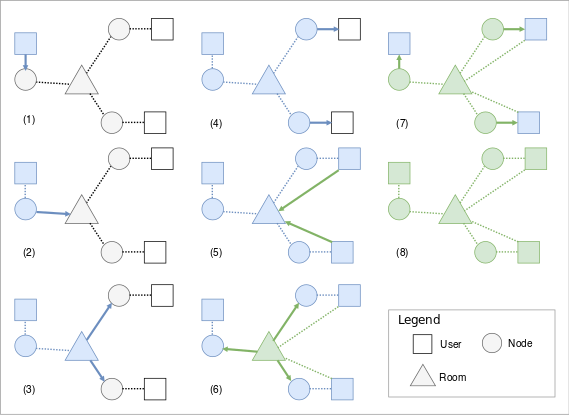
\includegraphics[width=\textwidth]{subfiles/img/diagram-final}
      \caption{A graphical representation of the process used by the Noble Eightfold Hash for verifiying and transmitting an \textsc{ehe} that updates the ledger in a patient room.}
      \label{fig:diagram}
    \end{center}
  \end{figure}

    \paragraph{Action 5: Post EHE Verification Key}
    Once the appropriate verified user has received a request, they must go into the room containing the u\textsc{ehe}, where it is now presented in the room ledger with a warning label indicating that it is unverified. The user must confirm that the \textsc{ehr} data that the u\textsc{ehe} is attempting to update is accurate.%

    Based on the contents of this data, one user, the majority of users, or, in some cases, every verified user must confirm the u\textsc{ehe} for verification. When this occurs, signature key(s) will be run through an encryption algorithm to confirm their authenticity. Once algorithm determines that the signature key(s) are authentic and owned by the appropriate verified user(s), the verification will be sent to the room to update the ledger and distribute the data. It is at the this point that a u\textsc{ehe} becomes a full-fledged \textsc{ehe}.%

    \paragraph{Action 6: Post Request for Room Ledger Distribution}
    Once the room has acknowledged verification of the \textsc{ehe}, the \textsc{ehe} will request an update to the ledger for that room. To do this, it will post a request to distribute the new room ledger to the nodes that the algorithm previously determined had appropriate verified associated users. It will also determine if there are any nodes that have verified users associated with the room that may not have been appropriate to sign the verification and post a request to those as well.%

    \paragraph{Action 7: Stage Update to Room Ledger}
    Once a node has received a request to distribute the new room ledger, it will then stage an updated version of the room ledger for the relevant users in preparation for the next time the user logs in.%

    \paragraph{Action 8: Distribute Electronic Health Record Data and Room Ledger}
    Until a user signs into DuraChain on a confirmed machine and accesses the room where the staged update is located, they will not have an updated version of the room ledger available to them. Upon sign-in, however, their version of the ledger will update and the \textsc{ehr} data will be accessible to them. Upon seeing a new \textsc{ehe} event in the room ledger, a user will know that this is a confirmed verified update to the Ledger and that the \textsc{ehr} data associated with the patient is the most up-to-date version.%

  \subsubsection{Benefits of Event-Based Distribution}
  Advances in event-based storage made by Matrix allow us to decentralize both records and conversations about a patient. This permits an unprecedented and patient-forward \textsc{dme} sales order life cycle that will save time and streamline the approach for getting equipment into the patient's home in a timely manner.%

  Event-based storage also scales readily, allowing for rapid, modular development and implementation of softwares beyond the \textsc{dme} application discussed here.%

  Using an event-based distribution model, stakeholders can interact in real time without the need to communicate with any of the centralized authorities that presently act as gatekeepers and bottlenecks. The real-time functional and spatial awareness enjoyed by all parties will lead to a greater understanding of where, when, and in what state any given sales order exists in its life cycle.%

  For our present \textsc{dme} implementation of \textsc{dlt}, our chief concern is providing data about the user(s). Currently, many actors in the \textsc{dlt} space are only concerned with dynamic content posting---live interaction, so to speak. Healthcare, however, is an excellent example of where static content posting is still alive and well.%

  In this regard, our system allows for a dynamic understanding of change as it acts on ``static'' content. By transmitting these variables as events, we can track who updates what details about a patient and thus use these data to track who is active inside a patient's room at any given time. The fine granularity offered by event-based information distribution will foster a deeper understanding of the patient care process.%

  %\paragraph{Servers as Synapses}
  %A useful analogy to conceptualize how the network of servers pass information back and forth is to imagine each connection as a synapse (the interface between neurons) in the brain. Neurons receive a stimulus and respond to that stimulus by taking an appropriate action or simply passing the input ``down the line.''%

  %In our network, a server will take an event posted by a user and fire it off to the rest of the servers it shares a connection with. The collective network then provides feedback about the broadcast by confirming and posting the event. Different servers fire off events that ripple throughout network of synapses and post to common spaces to inform the other servers that they have done so.%

\subsection{Implementation}
 Successful implementation of the DuraChain environment requires active adoption and participation by \textsc{dme} providers, who constitute our main client base.%

 In order to bring a client into our environment, they must have a copy of our server software properly installed and attached to their domain. From there, they can access our environment via our custom \textsc{ui} and begin creating patient rooms. To join a previously-existing patient room, they must be invited to an appropriately credentialed user inside of that room.%

\subsubsection{Protected Health Information}
Any discussion of healthcare data must obligatorily address the topic of Protected Health Information (\textsc{phi}). For DuraChain to be implemented properly, compliance with the Health Insurance Portability and Accountability Act of 1996 (\textsc{hipaa})\cite{HIPAA} is absolutely mandatory for both users and the servers housing patient data.%

By placing the server instances within the domain of the \textsc{dme} provider, the client assumes responsibility for creating users, patient rooms, and \textsc{hipaa} compliance more broadly. As the vendor of the DuraChain software, we assume liability only for performing due diligence on our clientele and extracting an assurance of their compliance with \textsc{hipaa}.%

In this way, the clients assume liability for compliance and removes that burden from us. This is not to a hedge or a dodge. In fact, it is actually the most efficient way to handle \textsc{hipaa} compliance and liability. Assuming that we only distribute our software to reputable and responsible \textsc{dme} businesses, who already have a \textsc{hipaa} mandate, then our software remains compliant as long as all server instances are maintained by compliant parties.%
